\documentclass[a4paper,11pt]{article}
\usepackage[utf8]{inputenc}
\usepackage[T1]{fontenc}
\usepackage[english]{babel}
\usepackage{amsmath,amssymb,amsthm,amsfonts}
\usepackage{graphicx} % REMOVE "demo" to include figures!
\usepackage{float,flafter}

\title{
	Computer Exercise 2\\
	EL2520 Control Theory and Practice
}
\author{
	Samuel Wintzell\\
	wintz@kth.se\\
	960522-1754
	\and
	Lucas Lov\'en \\ lucassl@kth.se  \\ 961126-2032
}

\newcommand{\image}[3][width=1.0\columnwidth]{
	\begin{figure}[h!]
		\centering
	    \includegraphics[#1]{#2}
		\caption{#3}
		\label{fig:#2}
	\end{figure}
}

\begin{document}
	\maketitle

	% Minimum phase case
	\section*{Minimum phase case}
  
    For the minimum phase case, the cross terms $\lambda_{12}$ of the Relative Gain Array are negative when evaluated at $\omega$ = 0. Hence we choose to pair $u_1$ and $y_1$,and $u_2$ and $y_2$. The
    controller $F(s)$ will thus be of the form:

    \[
    F(s)=
    \begin{bmatrix}
      f_1(s) & 0      \\
      0      & f_2(s) \\
    \end{bmatrix}
    \]
    where $f_i = K_i (1 + \dfrac{1}{T_i s})$, $i \in \{1,2\}$. The computed controller was:
    \[
    F(s)=
    \begin{bmatrix}
     \frac{9.904s + 1.678}{5.904s} & 0      \\
      0      & \frac{12.87s + 2.014}{6.391s} \\
    \end{bmatrix}
    \]

    \begin{figure}[H]
        \centering
        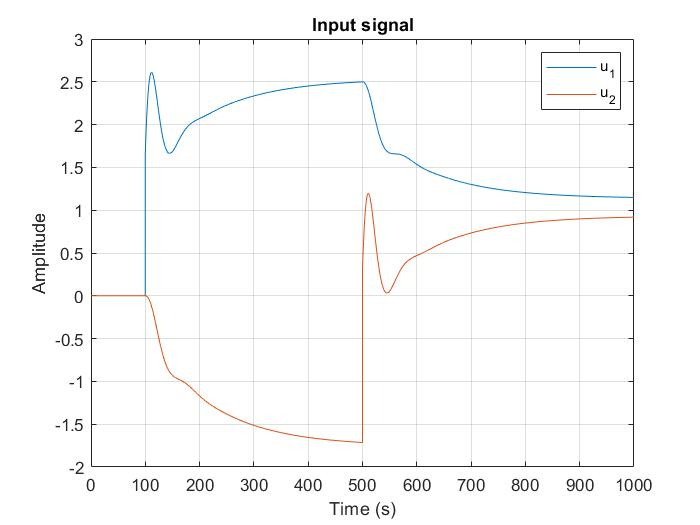
\includegraphics[width=0.8\linewidth]{minphase_simulink_u.jpg}
        \caption{Control signal}
        \label{f1}
    \end{figure}
    \begin{figure}[H]
        \centering
        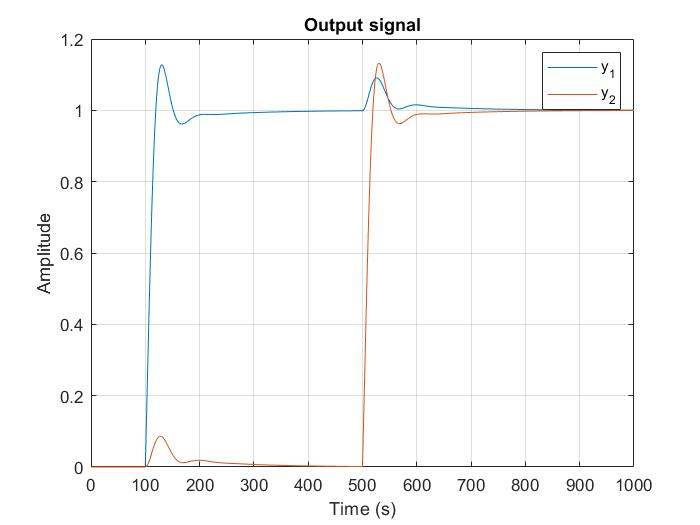
\includegraphics[width=0.8\linewidth]{minphase_simulink_y.JPG}
        \caption{Output signal}
        \label{f2}
    \end{figure}
    \begin{figure}[H]
        \centering
        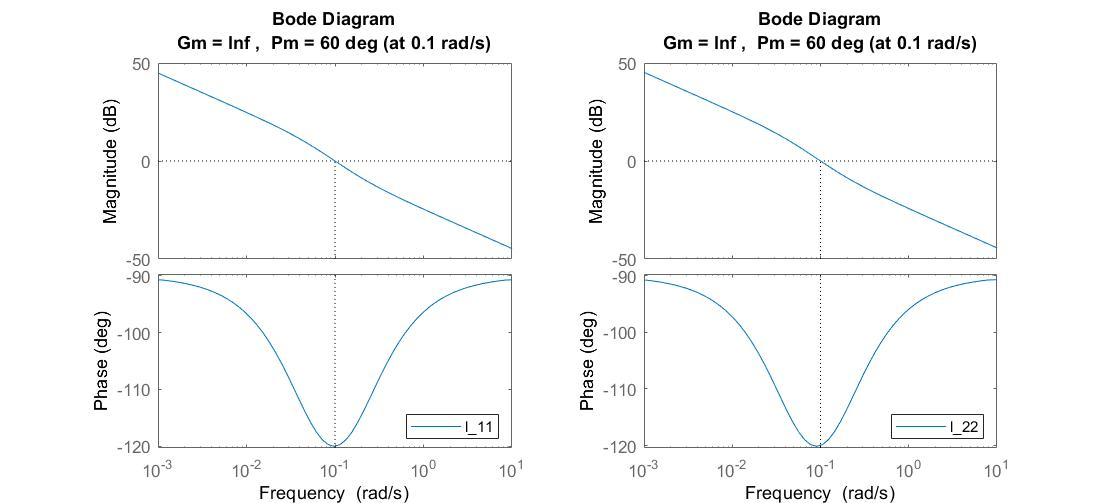
\includegraphics[width=1\linewidth]{minphase_L.jpg}
        \caption{Bode diagram of the loop gain $L(s)$. $l_{11}= left$ and $l_{22}=right$}
        \label{f3}
    \end{figure}
    
	Is the controller good?
	\\Looking at figure 2, control performance looks good. The system converges quickly after each step input and the loop gain satisfies both desired phase margin and cross-over frequency.\\\\
	Are the output signals coupled?\\
	As the step response plots from $u_1$ to $y_2$ and from $u_2$ to $y_1$ in G(s) suggests, the signals are coupled. On top of that the cross terms $g_{12}$ and $g_{21}$ are non-zero which reinforces the conclusion. 

	% Non-minimum phase case
	\section*{Non-minimum phase case}

    For the non-minimum phase case, the terms $\lambda_{11}$ and  $\lambda_{}22$ of the Relative Gain Array are negative when evaluated at s = 0. Hence we choose to pair $u_1$ with $y_2$ instead, and $u_2$ with $y_1$. The controller $F(s)$ will thus be of the form:

    \[
    F(s)=
    \begin{bmatrix}
      0 & f_1(s)      \\
      f_2(s)      & 0 \\
    \end{bmatrix}
    \]
    where $f_i = K_i (1 + \dfrac{1}{T_i s})$, $i \in \{1,2\}$.The computed controller was:
    \[
    F(s)=
    \begin{bmatrix}
     0 & \frac{0.6915s + 0.1437}{4.811s}      \\
      \frac{0.5792s + 0.1469}{3.943s}      & 0 \\
    \end{bmatrix}
    \]

	\begin{figure}[H]
        \centering
        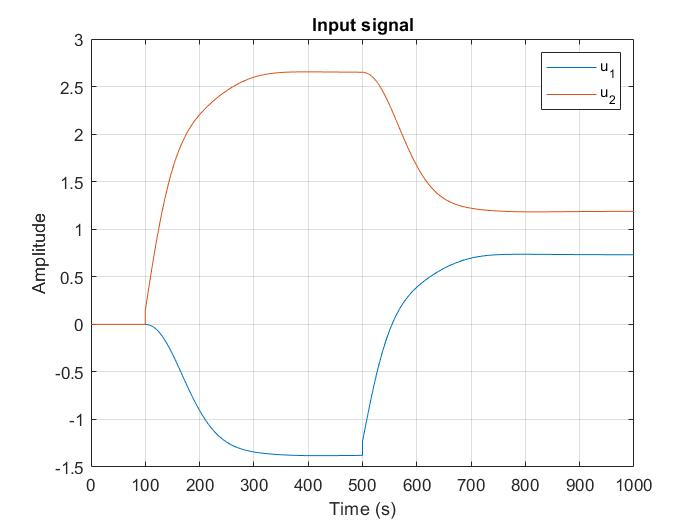
\includegraphics[width=0.8\linewidth]{nonminphase_simulink_u.jpg}
        \caption{Control signal}
        \label{f4}
    \end{figure}
    \begin{figure}[H]
        \centering
        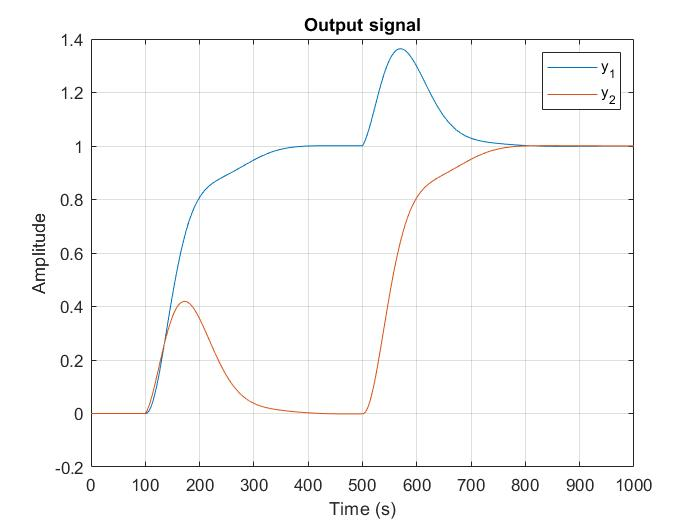
\includegraphics[width=0.8\linewidth]{nonminphase_simulink_y.jpg}
        \caption{Output signal}
        \label{f5}
    \end{figure}
    \begin{figure}[H]
        \centering
        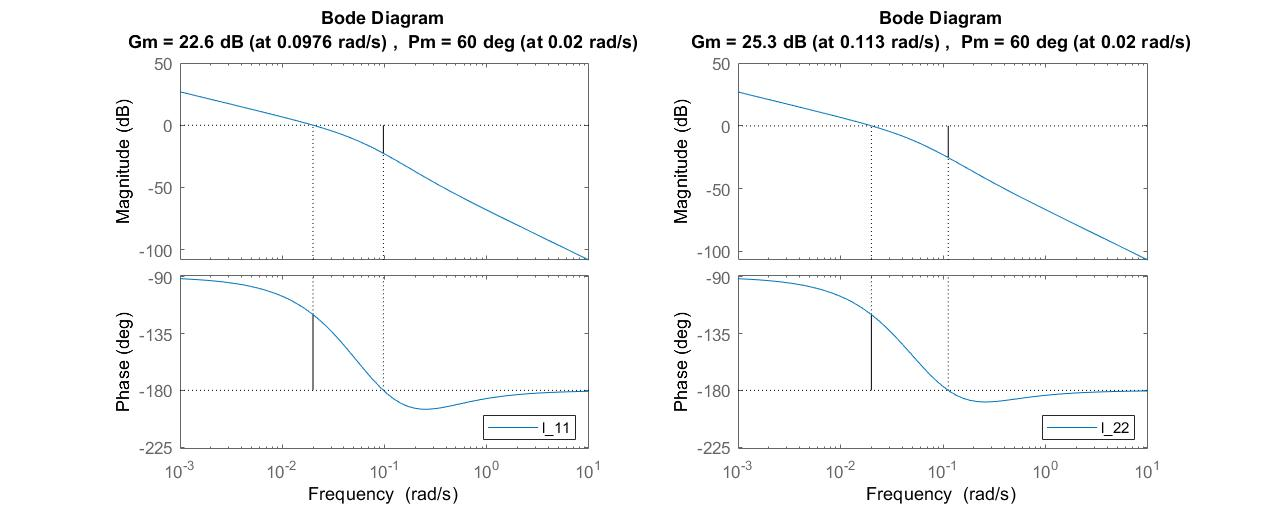
\includegraphics[width=1\linewidth]{nonminphase_L.jpg}
        \caption{Bode diagram of the loop gain $L(s)$. $l_{11}= left$ and $l_{22}=right$}
        \label{f6}
    \end{figure}
	Is the controller good?
	\\Comparing output signal plots from both cases it is clear that the control in the non-minimum phase performs worse. Performance is not very good. It is slow, but the system still converges. From the bode diagram in figure \ref{f6} we note that the loop gain has the desired phase margin and cross-over frequency.\\\\
	Are the output signals coupled?
	\\As can be seen in figure \ref{f5}, the output signals are coupled. Both outputs react to both inputs. Worth noting is that the effects are quite a bit worse in the non-minimum phase case. 

\end{document}
